\chapter{chapter1}
\songti
% 页码数字编号
\pagenumbering{arabic}
% 页码重新编号
\setcounter{page}{1}

chapter1
\chapter{chapter2}
chapter2

\section{section2.1}
section2.1

\begin{figure}[H]
	\centering
	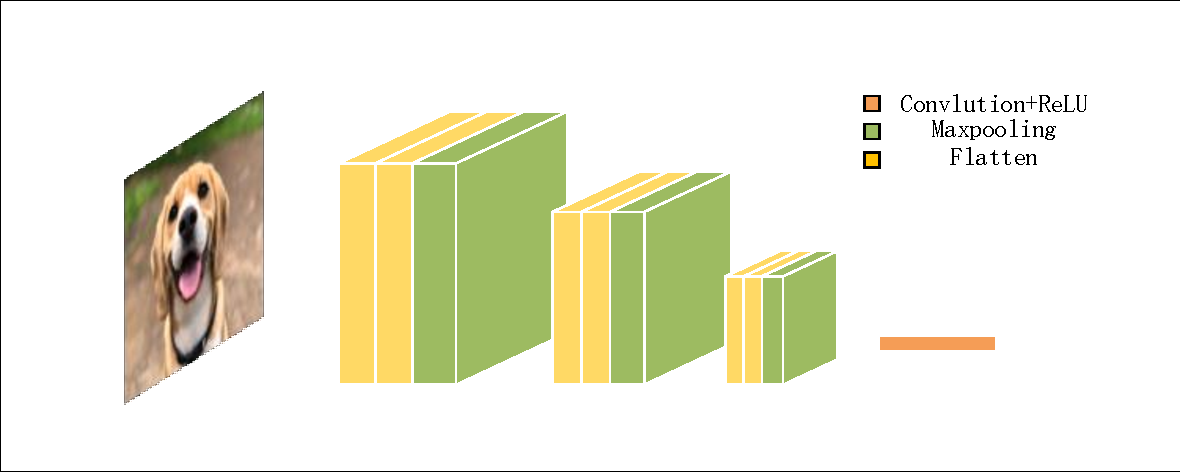
\includegraphics[width=120mm]{image/img02.pdf}
	\caption{caption1}
\end{figure}



\chapter{chapter3}
chapter3

% [H] 固定图片位置
\begin{figure}[H]
	\centering
	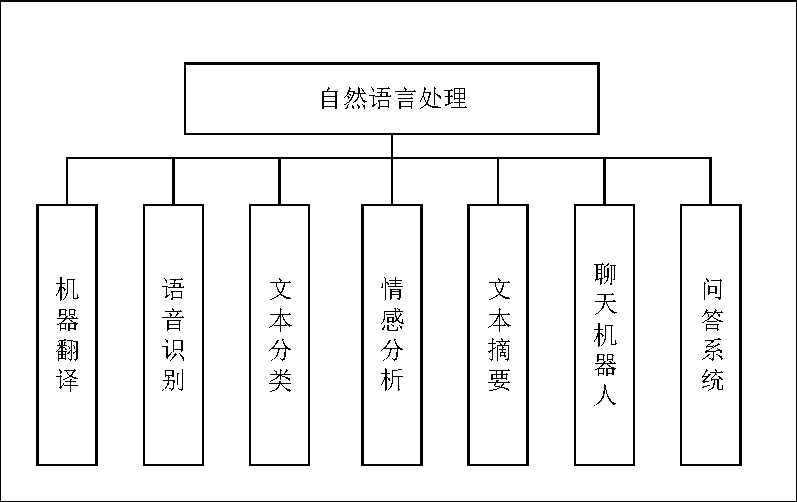
\includegraphics[width=120mm]{image/img03.pdf}
	\caption{cpation2}
\end{figure}




\chapter{chapter4}
\section{section4.1}


% 带标号equation
\begin{equation}
	w^* = \mathop{\arg\min}\limits_{\theta} \sum\limits_{i} L(y_i, f(x_i;w)) + \lambda\Omega(w)
\end{equation}


\section{section4.2}

设$ A\in C_r^{m \times n} $, $ \lambda_i $, $ r = rank(A) $, $ \lambda_i $  是$ A A^H $的特征值,$ \mu_i $是$ A^H A $的特征值,它们都是实数。且设
\begin{displaymath}
	\lambda_1 \geq \lambda_2 \cdots \geq \lambda_r > \lambda_{r+1} = \lambda_{r+2} = \cdots=\lambda_m = 0
\end{displaymath}
\begin{displaymath}
	\mu_1 \geq \mu_2 \cdots \geq \mu_r > \mu_{r+1} = \mu_{r+2} = \cdots = \mu_m = 0
\end{displaymath}

则特征值$ \lambda_i $与$ \mu_i $之间的关系为:$ \lambda_i = \mu >0,(i=1,2,\cdots,r) $。

设$ A\in C_r^{m \times n} $, $ A A^H $ 的正特征值 $ \lambda_i $, $ A^H A $ 的正特征值 $ \mu_i $, 称 $ \alpha_i = \sqrt{\lambda_i} = \sqrt{\mu_i} $, $ (i = 1, 2,\cdots,r) $ 是 $ A $ 的正奇异值,简称奇异值。若 $ A $ 是正规矩阵,则 $ A $ 的奇异值是A的非零特征向量的模长。

若$ A\in C_r^{m \times n} $, $ \delta_1 \geq \delta_2 \geq \cdots \geq \delta_r $ 是 $ A $ 的$ r $个正奇异值,则存在$ m $阶酉矩阵$ U $和$ n $阶酉矩阵$ V $,满足:
% 不带标号equation
\begin{displaymath}
	A = UDV^H = U \begin{bmatrix} \Delta & 0 \\ 0 & 0 \end{bmatrix} V^H
\end{displaymath} 
其中, $ \Delta = diag(\delta_1,\delta_2,\cdots,\delta_r) $, $ \Delta $ 为奇异对角阵,$ U $满足$ U^H A A^H U$是对角阵,$ V $满足 $ V^H A^H AV $是对角阵。$ U $的第$ i $列为$ A $的对应于$ \delta_i $ 奇异值对应的左奇异向量,$ V $的第$ i $列为$ A $的对应于$ \delta_i $奇异值对应的右奇异向量。它们的每一列均为单位向量,且各列之间相互正交。

若$ A\in C_r^{m \times n} $, $ \delta_1 \geq \delta_2 \geq \cdots \geq \delta_r $ 是 $ A $ 的$ r $个正奇异值,则总有次酉矩阵$ U_r \in U^{m \times r}_r, V_r \in V^{n \times r}_r$ 满足: $ A = U_r \Delta V_r^H $, 其中 $ \Delta = diag(\delta_1,\delta_2, \cdots, \delta_r) $。


\begin{displaymath}
	A = UDV^H = U\begin{bmatrix} \Delta & 0 \\ 0 & 0 \end{bmatrix} V^H = \sum^r_{i=1} A_i = \sum^r_{i=1}\delta_i u_i v_i^H
\end{displaymath}
